\documentclass[]{beamer}
\usepackage{pgfpages}

\setbeameroption{show notes on second screen}

\graphicspath{{../thesis/Figures/}}  % Location of the graphics files (set up for graphics to be in PDF format)

% Include any extra LaTeX packages required
\usepackage[]{biblatex}
\addbibresource{../thesis/library.bib}
\addbibresource{../thesis/inhand.bib}
\addbibresource{../thesis/webs.bib}

\usepackage{multicol}
\usepackage{booktabs}

\usetheme{metropolis}
\title{Autonomous Navigation Behaviors \\ for an \\ Aerial Robotics Software Framework}
\author{Guillermo Echegoyen Blanco \\ Technical University of Madrid}
\institute{
  \vspace{1cm}
  
\includegraphics[width=1.25cm]{logoFi.png}
  \hspace{7.5cm}
  
\includegraphics[width=1cm]{logoupm.png}
}
\date{\the\year}

\def\mAlertSpace{\vspace{0.5em}}
\def\mOrangeItem{\item[\textcolor{orange}{\textbullet}]}
\newcommand{\mSlideTitle}{{{\color{gray}\secname}} \# \subsecname}

\begin{document}

\maketitle

\begin{frame}{Overview}
  \begin{multicols}{2}
    \setbeamertemplate{section in toc}[sections numbered]
    \tableofcontents[hideallsubsections]
  \end{multicols}
\end{frame}

\section{Introduction}
\subsection{Motivation}
\begin{frame}{\mSlideTitle}
  \begin{alertblock}{Autonomous Navigation}
    \mAlertSpace%
    Move a drone through an automatically-generated, obstacle-free trajectory to a given point.
    \begin{itemize}
      \item Planning
      \item Localization
      \item Mapping
    \end{itemize}
  \end{alertblock}
\end{frame}

\subsection{Objectives}
\begin{frame}{\mSlideTitle}
  As a \alert{general goal} we want to:
  \begin{itemize}
    \item Construct an indoor \emph{Autonomous Navigation} interface inside Aerostack using a \textbf{lidar} sensor.
  \end{itemize}
  We propose the use of different state of the art algorithms following the Aerostack framework. The \alert{specific goals} are:
  \begin{itemize}
    \item Contribute to the research community
    \item Test implementation suitable for real time aerial robotics applications.
  \end{itemize}
\end{frame}

\section{Problem Description}
\subsection{Aerostack}
\begin{frame}{\mSlideTitle}
  General purpose, modular software framework for aerial robotics.
  \begin{figure}[ht]
    \centering
    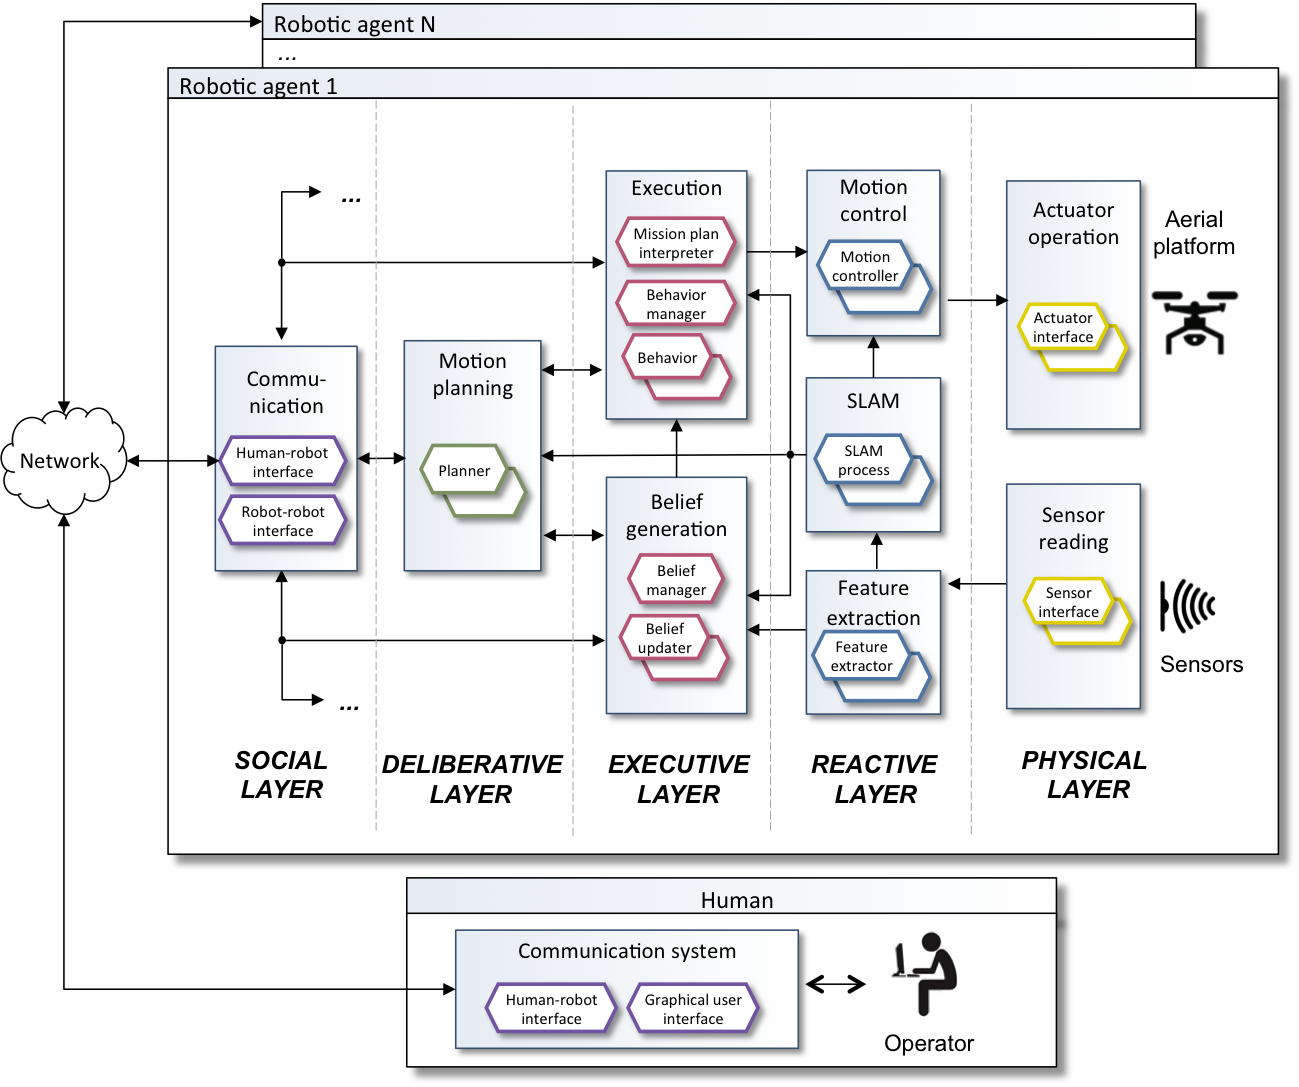
\includegraphics[height=0.7\textheight]{AerostackArquitecture.png}
    \caption{The Aerostack architecture}
  \end{figure}
\end{frame}

\subsection{Description}
\begin{frame}{\mSlideTitle}
  \begin{alertblock}{Aerostack}
    \mAlertSpace%
    Current version features:
    \begin{itemize}
      \item Planner: 2D geometric.
      \item Localization: Odometry, Aruco (\emph{requires preparation})
      \item Mapping: Hardcoded in the robot.
    \end{itemize}
  \end{alertblock}
\end{frame}

\subsection{Improvements}
\begin{frame}{\mSlideTitle}
  To provide an \textbf{autonomous}, \textbf{lidar} based navigation interface we propose:
  \begin{itemize}
    \mOrangeItem A module to localize and map using \textbf{lidar} sensor.
    \mOrangeItem A module to generate obstacle-free trajectories using that map.
    \mOrangeItem A module to follow a given trajectory.
  \end{itemize}
\end{frame}

\section{State of the Art}
\subsection{Localization}
\begin{frame}{\mSlideTitle}
  Usually based on trilateration.
  \begin{alertblock}{Outdoor Localization}
    \mAlertSpace%
    External sources:
    \begin{itemize}
      \item GSM Antennas
      \item Satellites
    \end{itemize}
  \end{alertblock}
  \begin{alertblock}{Indoor Localization}
    \mAlertSpace%
    Landmarks, beaconing (can provide more information)
    \begin{itemize}
      \item Bluetooth
      \item WiFi
    \end{itemize}
  \end{alertblock}
  In general, preparation of the environment is required.
\end{frame}

\note{%
  Bluetooth beacons are used in conferences and hotels to provide useful information.
}

\subsection{SLAM}
\begin{frame}{\mSlideTitle}
  With \alert{S}imultaneous \alert{L}ocalization \alert{a}nd \alert{M}apping, the robot constructs a map and localizes inside it at the same time.

  Does not require environment preparation.
  \begin{itemize}
    \mOrangeItem EKF Slam
    \mOrangeItem Particle Filters
    \mOrangeItem Graph Optimization
    \mOrangeItem \alert{Lidar Slam}
    \mOrangeItem Visual Slam
  \end{itemize}
\end{frame}

\note{%
  \begin{itemize}
    \item EKF: classic, intractable
    \item Particle Filters: Currently in use, fast, does not escale well for big maps
    \item Graph Optimization: Currently in use, very fast
    \item Lidar: the one we will use, fast and escalable
    \item Visual: SOTA orb slam, very interesting, requires large dictionary of words
  \end{itemize}
}

\subsection{Lidar Slam}
\begin{frame}{\mSlideTitle}
  Use a \textbf{lidar} sensor to do SLAM (Hector Slam \cite{hector_slam}).
  \begin{itemize}
    \item Ray traces alignment as a Gauss-Newton minimization problem.
    \item Multi resolution occupancy grid map.
    \item Already available as ROS node.
    \item Suitable for real time
    \item Realiable enough
  \end{itemize}
\end{frame}

\note{%
  \begin{itemize}
    \item Navigation system: interpolates IMU with SLAM, giving 3D, 6DOF
    \item 2D SLAM
  \end{itemize}
  It handles 3D with 6DOF by using a navigator that interpolates the IMU with the SLAM data.
  As a hill climbing algorithm (gradient ascent), it can get stuck in local minima, therefore, multiresolution occupancy grid map is used. Each coarser map have half the resolution of the preceding one, like in CV image pyramid problem. Instead of downsampling, the maps are kept in memory and simultaneously updated with the pose estimates of the alignment process.
}

\subsection{Hector Slam}
\begin{frame}{\mSlideTitle}
  \vspace{2.0em}
  \begin{columns}
    \column{0.60\textwidth}
      \begin{figure}
        \centering
        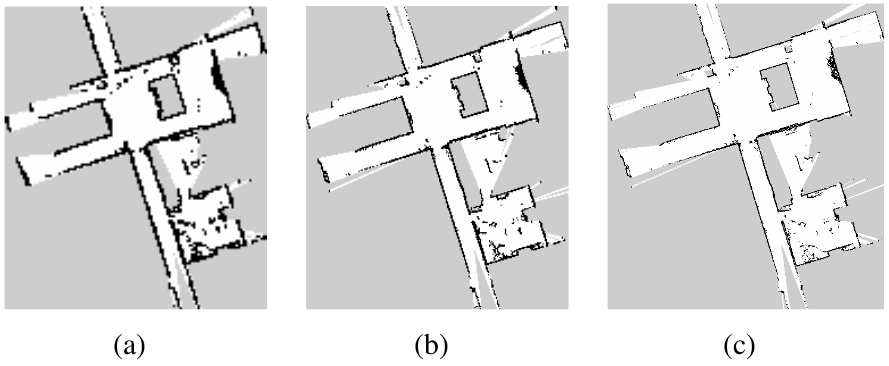
\includegraphics[width=1.05\textwidth]{HectorMultiRes.png}
        \caption{Multiresolution representation of the map}
      \end{figure}
    \column{0.40\textwidth}
      \begin{figure}
        \centering
        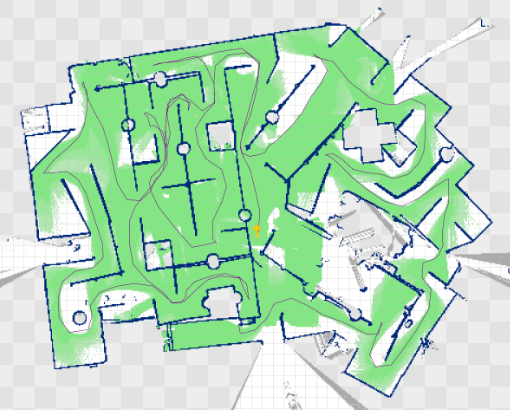
\includegraphics[width=0.9\textwidth]{HectorMap.png}
        \caption{Vehicle experiments: Learned map during a competition}
      \end{figure}
  \end{columns}
  \vspace{3.0em}
  Both images taken from \cite{hector_slam}
\end{frame}

\subsection{Planning}
\begin{frame}{\mSlideTitle}
  Lots of planning algorithms:
  \begin{columns}[T,onlytextwidth]
    \column{0.48\textwidth}
      \begin{figure}
        \centering
        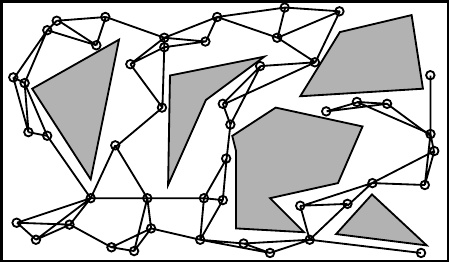
\includegraphics[width=\textwidth]{ProbRoadmap.jpg}
        \caption{Probabilistic roadmaps (taken from \cite{choset2005a})}
      \end{figure}
    \column{0.48\textwidth}
      \begin{figure}
        \centering
        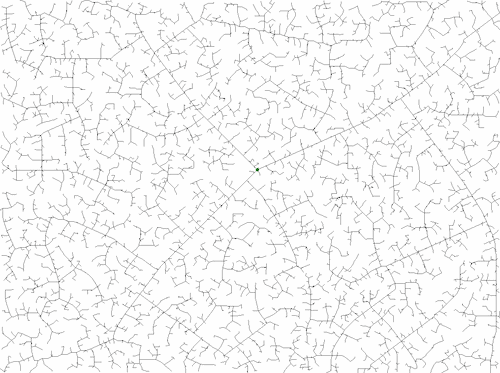
\includegraphics[width=\textwidth]{RRT.png}
        \caption{Rapidly exploring Random Trees (taken from \cite{wikipedia_rrts_web})}
      \end{figure}
  \end{columns}
\end{frame}

\note{%
  ToDo := Comment algorithms and ?redo slide to include planners as text and figures as rows?
  Say something about both algorithms
}

\subsection{Elastic Band Planner}
\begin{frame}{\mSlideTitle}
  Already available as a ROS module (\textbf{\emph{move base}})
  \begin{figure}
    \begin{columns}[T,onlytextwidth]
      \begin{column}{0.6\textwidth}
        \centering
        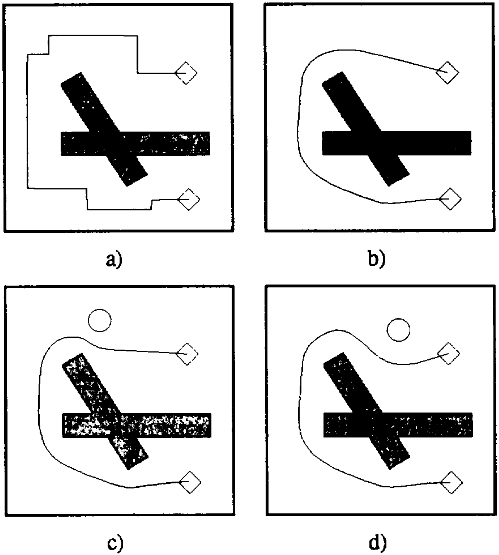
\includegraphics[width=0.8\textwidth]{Eband.png}
      \end{column}
      \begin{column}{0.4\textwidth}
        \vspace{2.0em}
        Pre planned path
        \begin{itemize}
          \item Forces applied
          \item Handle moving obstacles
        \end{itemize}
        In c) and d) an obstacle moves and the path is deformed.
      \end{column}
    \end{columns}
    \caption{Elastic Band with a moving obstacle (taken from \cite{eband})}
  \end{figure}
\end{frame}

\section{Implementation}
\subsection{ROS}
\begin{frame}{\mSlideTitle}
  \alert{R}obot \alert{O}perating \alert{S}ystem. Widely used in robotics research.
  \begin{itemize}
    \mOrangeItem Pub-Sub architecture (topics \& services).
    \mOrangeItem Multiple programming languages (C, C++, Python\dots)
    \mOrangeItem Logic encapsulation
  \end{itemize}
\end{frame}

\note{%
  \begin{itemize}
    \item There is a master server which proxies messages from and to publishers subscribers
    \item Algorithms can be encapsulated inside an isolated process that acts as a pub or sub
    \item Provides modularity and testability
  \end{itemize}
}

\subsection{Aerostack}
\begin{frame}{\mSlideTitle}
  Aerostack features:
  \begin{itemize}
    \mOrangeItem ROS node
    \mOrangeItem Robot processes.
    \mOrangeItem \alert{Behavior} processes.
  \end{itemize}
\end{frame}

\note{%
  \begin{itemize}
    \item ROS: Lowest level processes. Drivers \& hardware.
    \item Robot process: Mid level process, general algorithms (like aruco recognition)
    \item Behavior: Highest level, algorithm monitor, useful to be coordinated.
  \end{itemize}
}

\subsection{Behavior System}
\begin{frame}{\mSlideTitle}
  The Behavior Manager coordinates the execution of all the behaviors. A behavior:
  \begin{itemize}
    \mOrangeItem Is the highest level abstraction component.
    \mOrangeItem Encapsulates an algorithm.
    \mOrangeItem Listens to \emph{start} and \emph{stop} events and emmits \emph{error} events.
    \mOrangeItem Can have \emph{exclusive constraints} and dependencies on other processes.
  \end{itemize}
\end{frame}

\subsection{Navigation Interface}
\begin{frame}{\mSlideTitle}
  Therefore, the following components should be provided as behaviors or robots processes:
  \begin{itemize}
    \mOrangeItem \alert{Behavior} to localize using lidar.
      \begin{itemize}
        \item Behavior \emph{Self Localize And Map by Lidar}
        \item Hector Slam ROS module (monitored by $\uparrow$)
      \end{itemize}
    \mOrangeItem \alert{Behavior} to navigate the drone to a certain pose.
      \begin{itemize}
        \item Behavior \emph{Go To Point}
        \item Behavior \emph{Follow Path}
        \item Behavior \emph{Generate Path}
      \end{itemize}
    \mOrangeItem \alert{Robot process} to plan obstacle-free trajectories using lidar.
      \begin{itemize}
        \item \emph{Path planner} robot \emph{process}
        \item Move base ROS module (monitored by $\uparrow$)
      \end{itemize}
  \end{itemize}
\end{frame}

\subsection{Implemented Behaviors}
\begin{frame}{\mSlideTitle}
  Implementing each behavior separately enables:
  \begin{itemize}
    \item Different, granular control over functionallity
    \item Testability of components
    \item Separation of functionallity.
  \end{itemize}
\end{frame}

\note{%
  \begin{itemize}
    \item This way a developer can use each module separately
    \item Enables fine control on Python missions
    \item Debugs each part separately
  \end{itemize}
}

\subsection{Behavior Self Localize And Map by Lidar}
\begin{frame}{\mSlideTitle}
  \begin{columns}
    \begin{column}{0.5\textwidth}
      \begin{itemize}
        \mOrangeItem Monitors the \emph{Hector Slam} ROS module
        \mOrangeItem Applies EKF to: IMU, Odometry, SLAM
        \mOrangeItem Instructs the Aerostack for localization and mapping.
      \end{itemize}
    \end{column}
    \begin{column}{0.5\textwidth}
      \begin{figure}
        \centering
        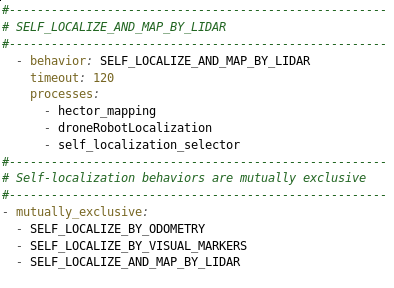
\includegraphics[height=0.4\textheight,keepaspectratio]{BehaviorSlamCatalog.png}
      \end{figure}
    \end{column}
  \end{columns}
  %\vspace{-1.2em}
  \begin{figure}
    \centering
    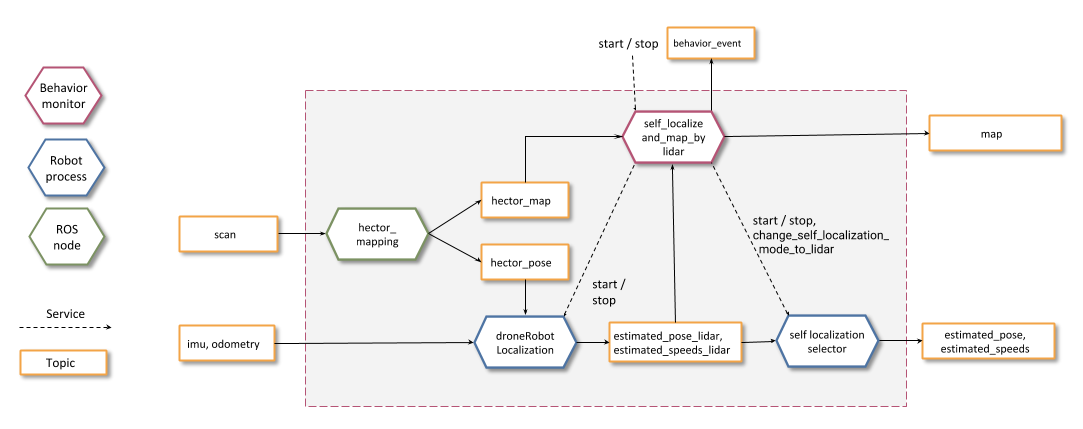
\includegraphics[width=0.8\textwidth]{BehaviorSlamArquitecture.png}
  \end{figure}
\end{frame}

\subsection{Behavior Go To Point in Occupancy Grid}
\begin{frame}{\mSlideTitle}
  \begin{columns}
    \hspace{0.5cm}
    \begin{column}{0.55\textwidth}
      Given a point:
      \begin{itemize}
        \mOrangeItem Gets an obstacle-free trajectory.
        \mOrangeItem Instructs the trajectory controller to move the drone.
        \mOrangeItem Replans if an obstacle arises in the way.
      \end{itemize}
      \begin{minipage}{0.65\textheight}
        \begin{figure}[!ht]
          \hspace{-2cm}
          \vspace{-2cm}
          \centering
          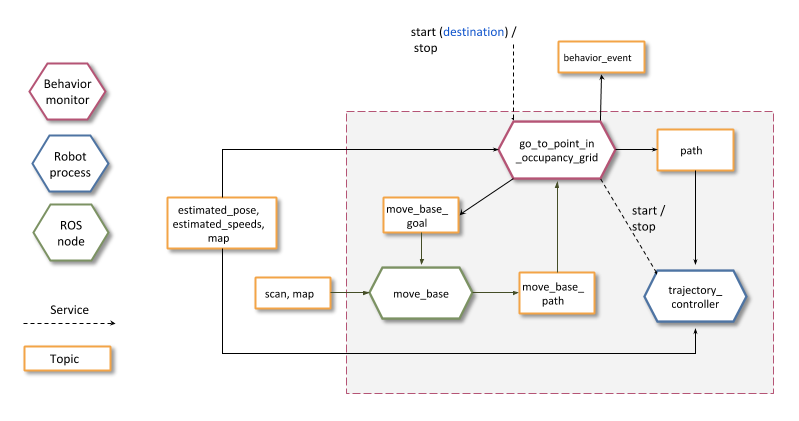
\includegraphics[width=1.5\textwidth,keepaspectratio]{BehaviorGTPArquitecture.png}
        \end{figure}
      \end{minipage}
    \end{column}
    \hspace{2.0cm}
    \begin{column}{0.45\textwidth}
      \begin{figure}
        \centering
        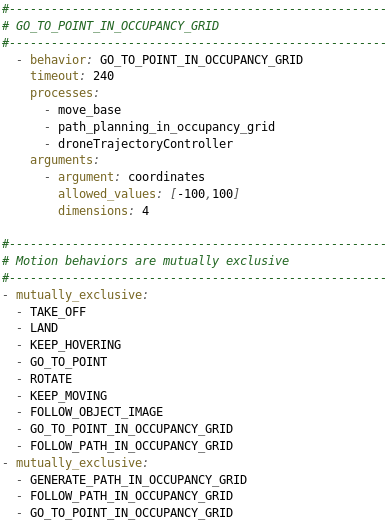
\includegraphics[width=0.8\textwidth,keepaspectratio]{BehaviorGTPCatalogVertical.png}
      \end{figure}
    \end{column}
  \end{columns}
\end{frame}

\subsection{Behavior Follow Path in Occupancy Grid}
\begin{frame}{\mSlideTitle}
  \begin{columns}
    \hspace{0.5cm}
    \begin{column}{0.55\textwidth}
      Given a path:
      \begin{itemize}
        \mOrangeItem Instructs the trajectory controller to move the drone.
        \mOrangeItem No obstacle avoidance is provided.
      \end{itemize}
      \begin{minipage}{0.65\textheight}
        \begin{figure}[!ht]
          \hspace{-2cm}
          \vspace{-2cm}
          \centering
          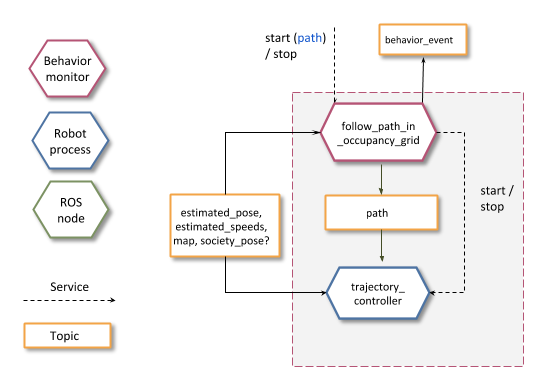
\includegraphics[width=1.5\textwidth,keepaspectratio]{BehaviorFPArquitecture.png}
        \end{figure}
      \end{minipage}
    \end{column}
    \hspace{1.5cm}
    \begin{column}{0.45\textwidth}
      \begin{figure}
        \centering
        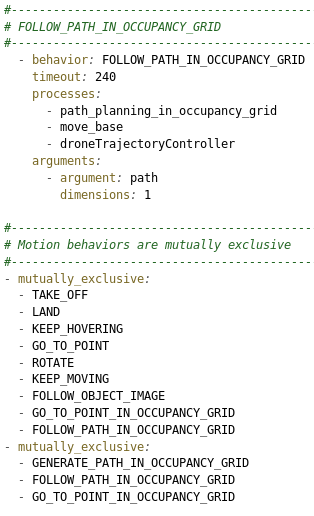
\includegraphics[width=0.7\textwidth,keepaspectratio]{BehaviorFPCatalogVertical.png}
      \end{figure}
    \end{column}
  \end{columns}
\end{frame}

\subsection{Behavior Generate Path in Occupancy Grid}
\begin{frame}{\mSlideTitle}
  \begin{columns}
    \begin{column}{0.5\textwidth}
      \vspace{1.2em}

      Given a point:
      \begin{itemize}
        \mOrangeItem Gets an obstacle-free trajectory.
        \mOrangeItem Stores the trajectory in the Belief Memory
      \end{itemize}
    \end{column}
    \begin{column}{0.5\textwidth}
      \begin{figure}
        \centering
        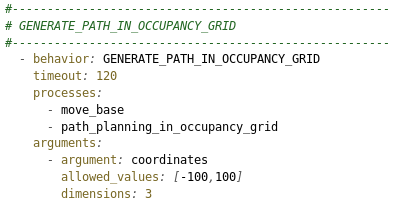
\includegraphics[height=0.3\textheight,keepaspectratio]{BehaviorGPCatalog.png}
      \end{figure}
    \end{column}
  \end{columns}
  %\vspace{-1.2em}
  \begin{figure}
    \centering
    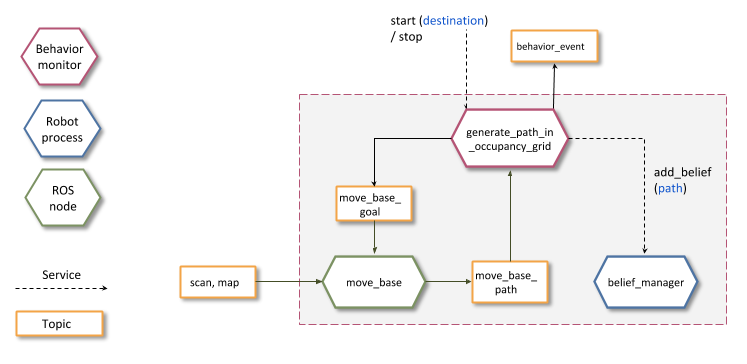
\includegraphics[width=0.8\textwidth]{BehaviorGPArquitecture.png}
  \end{figure}
\end{frame}

\section{Experiments}
\begin{frame}{\secname}
  \alert{Boiler inspection mission}
  \begin{figure}
    \centering
    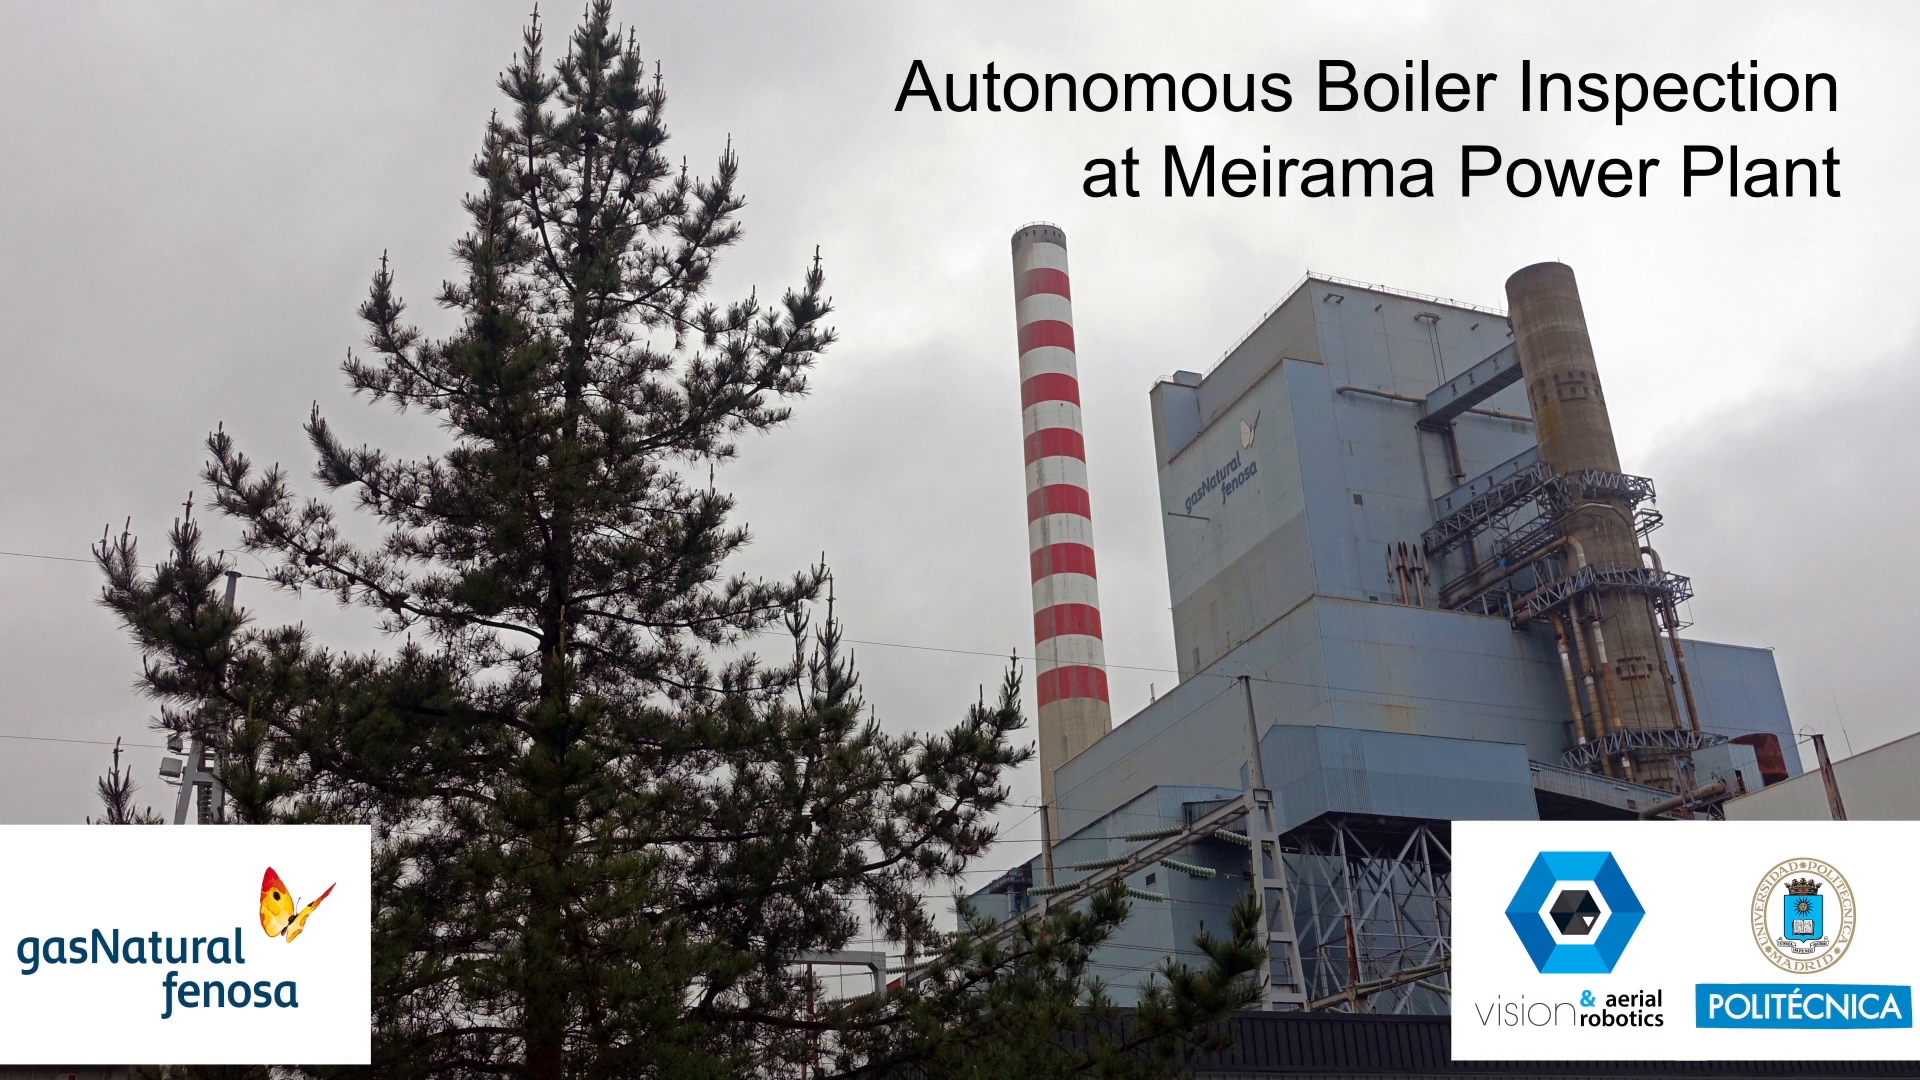
\includegraphics[width=0.8\textwidth]{BoilerReal.png}
  \end{figure}
\end{frame}

\subsection{Experiment Details}
\begin{frame}{\mSlideTitle}
  Boiler mission both in simulation and real flight:
  \vspace{2.5em}
  \begin{columns}
    \begin{column}{0.5\textwidth}
      Simulation
      \begin{itemize}
        \item Gazebo + RotorS simulator
        \item Hummingbird Drone
        \item 16x16x57 - WxDxH mts
      \end{itemize}
    \end{column}
    \begin{column}{0.5\textwidth}
      Real Flight
      \begin{itemize}
        \item Sports Center
        \item DJI 100 Matrice Drone
        \item 10x25x14 - WxDxH mts
      \end{itemize}
    \end{column}
  \end{columns}
\end{frame}

% ToDo := Remove this slide?
\subsection{Simulated Experiment}
\begin{frame}{\mSlideTitle}
  \begin{figure}
    \centering
    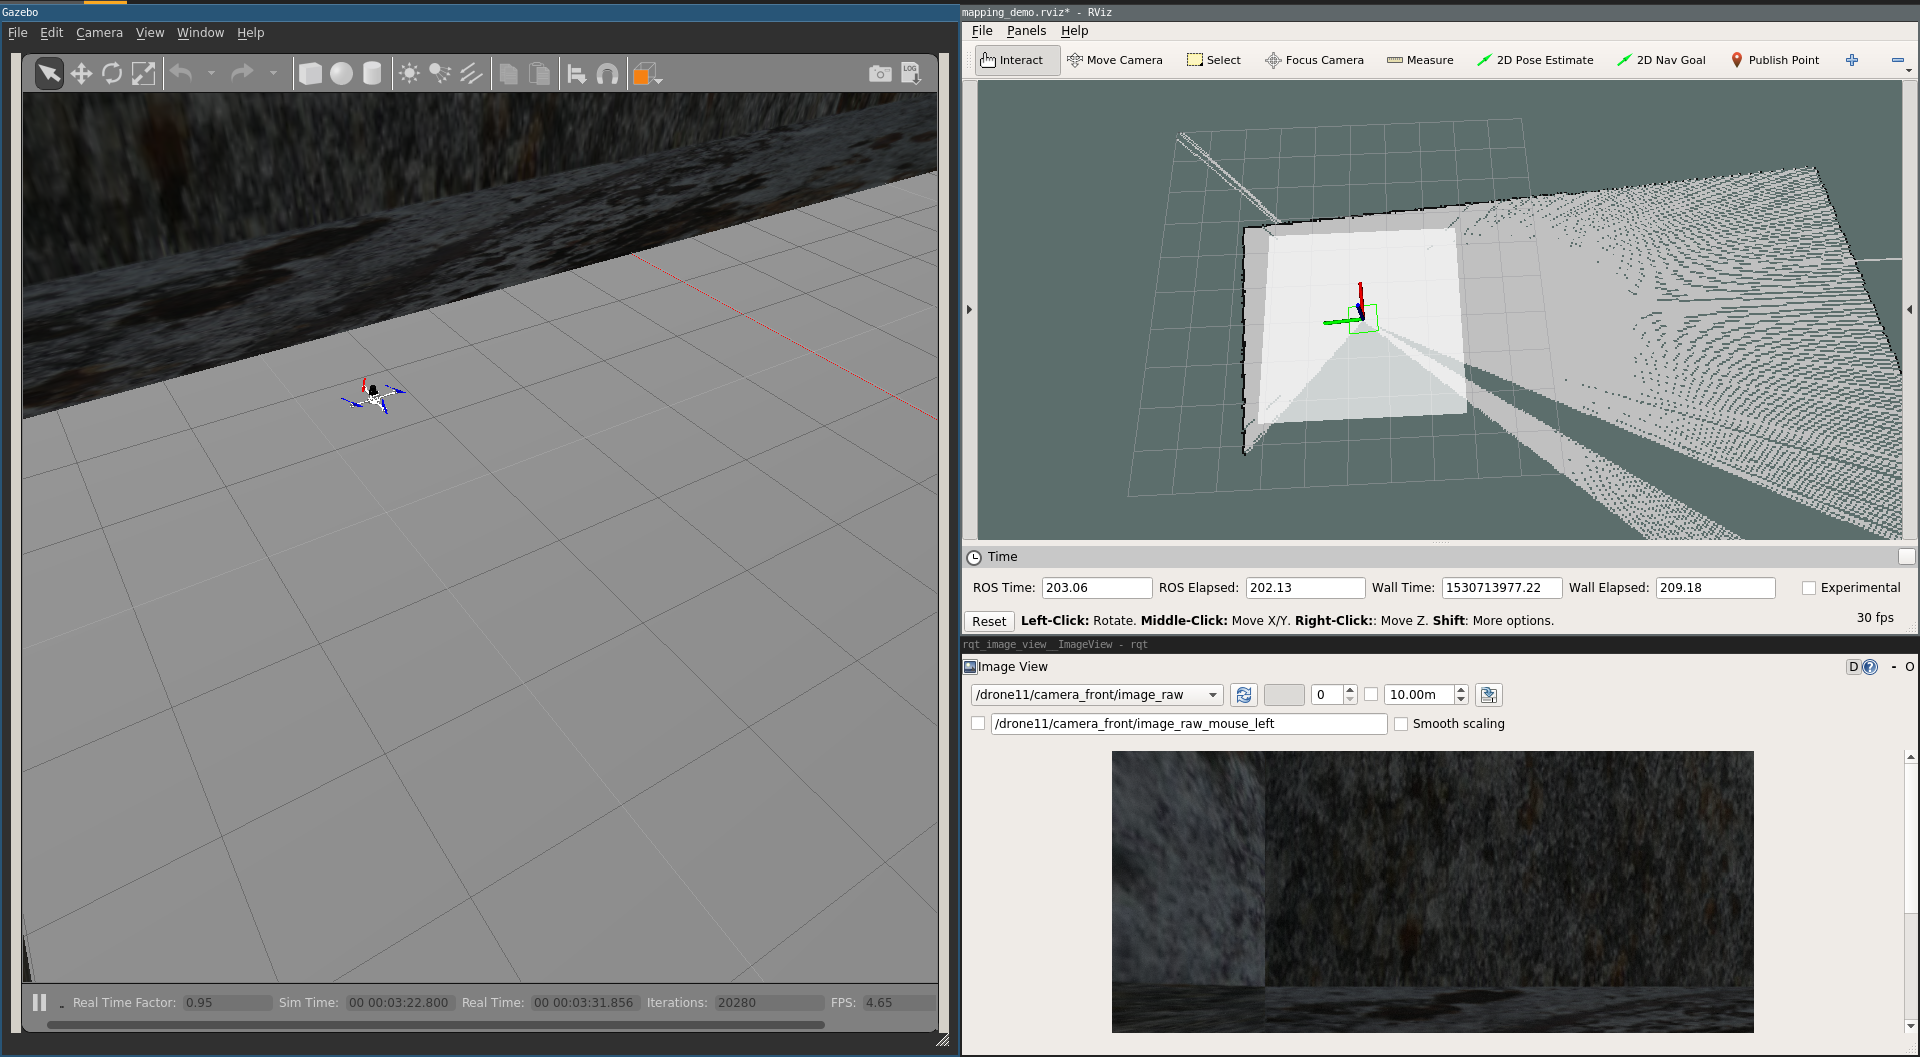
\includegraphics[width=0.9\textwidth]{FullSim.png}
    \caption{Simulated boiler environment}
  \end{figure}
\end{frame}

% ToDo := Remove this slide?
\subsection{Real Experiment}
\begin{frame}{\mSlideTitle}
  \begin{figure}
    \centering
    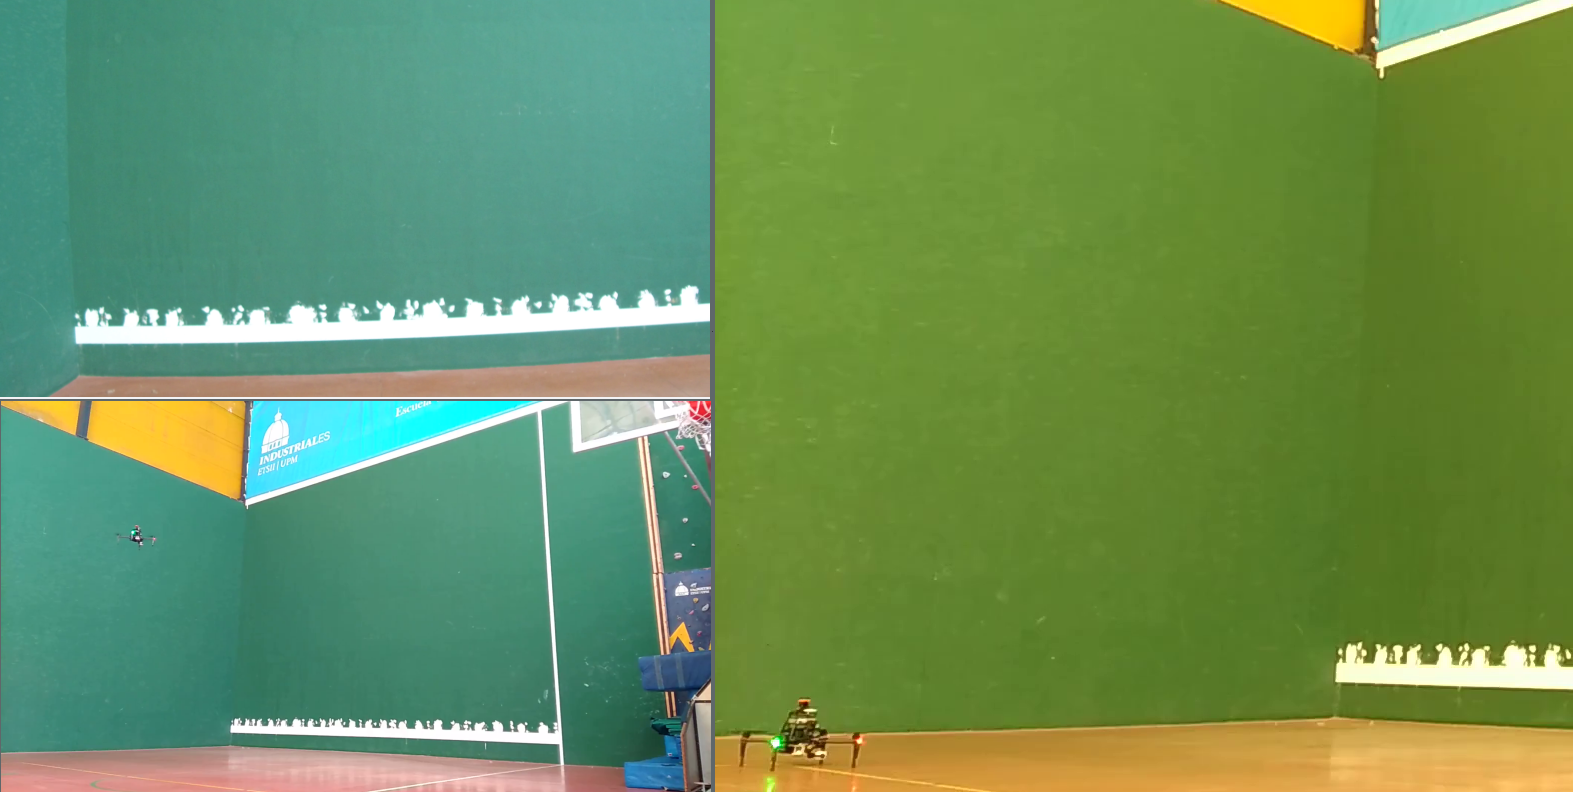
\includegraphics[width=0.9\textwidth]{RealFlight.png}
    \caption{Real experiment on the Sports center (\href{run:real_flight.mp4}{\color{blue}{video}})}
  \end{figure}
\end{frame}

\subsection{Data}
\begin{frame}{\mSlideTitle}
  \begin{table}
  \centering
  \begin{tabular}{lccr}
    \multicolumn{4}{c}{\textit{Simulation}}                         \\ \hline
    \textit{\#} & \textit{Correct} & \textit{Avg. Total Point} & \textit{Avg. Time} \\ \bottomrule
    \textit{Go to Point} & 41/60 (0.68\%) & 1.82 ($\pm$ 0.52) & 11.43 ($\pm$ 3.12) \\ \bottomrule
    \textit{Follow Path} & 39/60 (0.65\%) & 1.97 ($\pm$ 0.59) & 12.21 ($\pm$ 3.58) \\ \bottomrule
    \textit{Generate Path} & 60/60 (100\%) & 0.20 ($\pm$ 0.00) & 1.20 ($\pm$ 0.01) \\ \bottomrule
    \hline
    \multicolumn{4}{c}{\textit{ }}                                  \\
    \multicolumn{4}{c}{\textit{Real Flight}}                        \\ \hline
    \textit{Go to Point} & 16/18 (0.88\%) & 0.94 ($\pm$ 0.23) & 5.97 ($\pm$ 1.38) \\ \bottomrule
  \end{tabular}
\end{table}

\end{frame}

\note{%
  \begin{itemize}
    \item Simulation has more tests
    \item EKF Localization worse in simulation
    \item Time adds up because of timeouts (bad loc)
  \end{itemize}
}

\subsection{Discussion}
\begin{frame}{\mSlideTitle}
  \begin{itemize}
    \mOrangeItem Much room for improvement
    \mOrangeItem Localization is not accurate enough (lots of timeouts)
    \mOrangeItem Real flight is more stable \& fast
    \mOrangeItem Simulation is more tested
  \end{itemize}
\end{frame}

\section{Conclusions}
\begin{frame}{\secname}
  With \dots
  \begin{itemize}
    \mOrangeItem Improve Localization
    \mOrangeItem Lower timeout
    \mOrangeItem Extend testing
  \end{itemize}
  \dots an \textbf{autonomous navigation can be achieved}.
\end{frame}

\begin{frame}[standout]
  Questions?
\end{frame}

\section{References}
\begin{frame}[allowframebreaks]{References}
  \printbibliography%
\end{frame}

\end{document}

